\newpage
\section{Exercises: Discrete Fourier Transform}

\begin{enumerate}
\item Let $x(t)$ be some continuous-time signal that we wish to sample. The signal is discretized with a sampling rate of $f_{s}=17$ kHz, giving a discrete-time signal $x[n]$ of length $N$. We apply a discrete Fourier transform to the discrete-time signal $x[n]$, giving the signal $\hat{x}[k]$. Here $n$ and $k$ are integers.

\begin{enumerate}[a)]
    \item What are the continuous-time frequencies $f_{k}$ (in hertz) that correspond to the spectral components of $\hat{x}[k]$?
    
    \item What value of $N$ gives a frequency resolution of $0.1$ Hz when analyzing the signal $x[n]$ using a DFT?
\end{enumerate}

\begin{marginfigure}
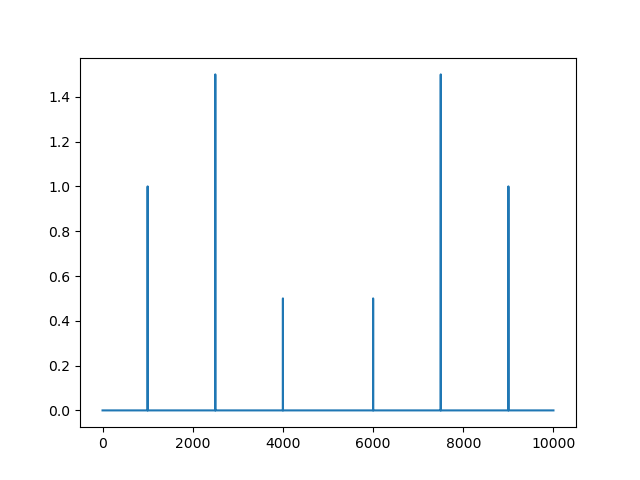
\includegraphics[width=7.0cm,height=6.8cm]{ch15/figures/ex152.png}
\caption{The magnitudes of six spectral components of the signal defined in Equation \ref{eq:ex15_2}}
\label{fig:ch15_ex15_2}
\end{marginfigure}

\item The code in Listing \ref{code:ex152} creates a discrete-time signal consisting of three sinusoidal signals:
\begin{equation}
x[n]=cos(\hat{\omega}_0 n)+2cos(\hat{\omega}_1 n)+3cos(\hat{\omega}_2 n)
\label{eq:ex15_2}
\end{equation}
and calculates the magnitude spectrum of this signal. The spectrum is shown in Figure \ref{fig:ch15_ex15_2}.

\lstinputlisting[language=Python,caption=Create a signal consisting of three sinusoids and analyze the magnitude spectrum,label=code:ex152,linerange={1-2,4-14}]{ch15/code/ex15_2.py}

\begin{enumerate}[a)]
    \item Show that frequencies $\hat{\omega}_0$, $\hat{\omega}_1$, and $\hat{\omega}_2$ in units of radians per sample correspond to frequencies $f_0=4000$, $f_1=1000$, and $f_0=2500$ in units of hertz.
    \item Show that signal $x[n]$ is periodic ($x[n]=x[n+N]$). Determine the fundamental period of this signal in samples and in units of seconds. 
    \item Modify the code so that the figure produced by the code, shown in Figure \ref{fig:ch15_ex15_2}, displays frequency on the horizontal axis units of hertz. Make sure that you plot both the positive and negative frequency components of the signal, recalling that a cosine signal consists of a positive and negative frequency complex sinusoidal signal. Verify that you get the correct frequency axis by looking at the relative magnitudes of the six non-zero frequency components of the signal. Hint: you may find Python functions \verb|numpy.fft.fftshift| and \verb|numpy.fft.fftfreq| useful for this exercise.
\end{enumerate}


\end{enumerate}
